\documentclass[12pt,a4paper]{article}

% ---------------------------------------------------------------------------
% Datos de la portada (modificar aquí)
% ---------------------------------------------------------------------------
\newcommand{\titulo}{Resolución del juego \textit{Lights Out} mediante sistemas de ecuaciones lineales con aritmética binaria}
\newcommand{\fecha}{14 de octubre de 2026}
\newcommand{\repositorio}{https://github.com/GuillermoRivero98/lights-out}

% ---------------------------------------------------------------------------
\usepackage[T1]{fontenc}
\usepackage[utf8]{inputenc}
\usepackage[spanish,es-noshorthands,es-tabla,es-nodecimaldot]{babel}
\usepackage{mathptmx}
\usepackage[margin=2.54cm]{geometry}
\usepackage{setspace}
\usepackage{amsmath,amssymb,amsthm}
\usepackage{graphicx}
\usepackage{booktabs,array,multirow}
\usepackage{caption}
\usepackage{float}
\usepackage{enumitem}
\usepackage{xcolor}
\usepackage{titlesec}
\usepackage{fancyhdr}
\usepackage[spanish,ruled,linesnumbered,vlined]{algorithm2e}
\usepackage[hidelinks]{hyperref}
\urlstyle{same}

\onehalfspacing
\setlength{\emergencystretch}{3em}
\setlength{\parindent}{1.27cm}
\setlength{\parskip}{0pt}

% Encabezados al estilo APA: nivel 1 centrado y en negrita, nivel 2 alineado
% a la izquierda en negrita, nivel 3 en negrita cursiva.
\titleformat{\section}{\centering\normalfont\bfseries}{\thesection.}{0.5em}{}
\titleformat{\subsection}{\normalfont\bfseries}{\thesubsection.}{0.5em}{}
\titleformat{\subsubsection}{\normalfont\bfseries\itshape}{\thesubsubsection.}{0.5em}{}
\titlespacing*{\section}{0pt}{1.2em}{0.6em}
\titlespacing*{\subsection}{0pt}{1em}{0.4em}

% Pies de figura debajo y títulos de tabla arriba (guía de informes).
\captionsetup{font=small,labelfont=bf,labelsep=period,justification=justified,singlelinecheck=false}
\captionsetup[table]{position=top,skip=6pt}
\captionsetup[figure]{position=bottom,skip=6pt}

\pagestyle{fancy}
\fancyhf{}
\fancyhead[R]{\thepage}
\renewcommand{\headrulewidth}{0pt}

\theoremstyle{plain}
\newtheorem{proposicion}{Proposición}
\theoremstyle{definition}
\newtheorem{definicion}{Definición}
\theoremstyle{remark}
\newtheorem*{observacion}{Observación}
\renewcommand{\qedsymbol}{$\blacksquare$}

\newcommand{\F}{\mathbb{F}_2}
\newcommand{\V}{V}
\newcommand{\codigo}[1]{\texttt{#1}}
% \@@input es expandible y permite insertar filas generadas dentro de tabular.
\makeatletter\newcommand{\filasdetabla}[1]{\@@input #1 }\makeatother
\SetAlgorithmName{Algoritmo}{algoritmo}{Lista de algoritmos}
\SetKwInOut{Entrada}{Entrada}
\SetKwInOut{Salida}{Salida}

\begin{document}

% ---------------------------------------------------------------------------
% Portada
% ---------------------------------------------------------------------------
\begin{titlepage}
\thispagestyle{empty}
\centering
\vspace*{3cm}
{\bfseries \titulo\par}
\vspace{2.5cm}
Guillermo Rivero (C.I. 5048260-2)\par
Enzo Barreto (C.I. 4523297-3)\par
\vspace{1.5cm}
Facultad de Ingeniería y Tecnologías, Universidad Católica del Uruguay\par
\vspace{0.5cm}
Álgebra Aplicada\par
\vspace{0.5cm}
\fecha\par
\end{titlepage}

% ---------------------------------------------------------------------------
\section*{Resumen}
% ---------------------------------------------------------------------------
\addcontentsline{toc}{section}{Resumen}

\noindent
\textit{Lights Out} es un juego de un tablero de $n\times n$ luces en el que presionar una luz cambia su estado y el de sus vecinas ortogonales; el objetivo es apagarlas todas. El objetivo de este trabajo es modelar las soluciones del juego como un sistema de ecuaciones lineales sobre el conjunto $\{0,1\}$ con suma binaria, e implementar en Python un método que lo resuelva. Primero se demuestra que ninguna luz necesita presionarse más de una vez y que el orden de las pulsaciones no altera el resultado, lo que permite representar cada solución con un vector de $n^2$ componentes binarias. Luego se construye el sistema $A\mathbf{x}=\mathbf{b}$, se justifica cada ecuación del ejemplo $3\times 3$ y se implementa la escalerización de Gauss-Jordan con suma binaria. La implementación se validó con los ejemplos dados y con 20\,000 tableros aleatorios para $n$ entre 1 y 10, comprobando por simulación cada solución obtenida. Los resultados muestran que la matriz del sistema es invertible para $n\in\{1,2,3,6,7,8,10\}$, pero no para $n\in\{4,5,9\}$, en cuyo caso solo una fracción $2^{-d}$ de los tableros tiene solución, siendo $d$ la dimensión del núcleo; las frecuencias observadas coinciden con ese valor. Además, se encontró que la escalerización sin intercambio de filas se detiene en el segundo paso para todo $n\geq 2$, por lo que el intercambio es necesario. Se concluye que el modelo lineal resuelve el juego de forma exacta y permite decidir de antemano si un tablero tiene solución.

\vspace{0.5em}
\noindent\textit{Palabras clave:} Lights Out, sistemas lineales, aritmética binaria, escalerización gaussiana, núcleo.

\newpage

% ---------------------------------------------------------------------------
\section{Introducción}
% ---------------------------------------------------------------------------

\textit{Lights Out} es un juego electrónico que se juega sobre un tablero cuadrado de $n\times n$ luces, cada una prendida o apagada. El juego parte de una configuración cualquiera y el jugador busca llegar al estado en que todas las luces están apagadas. La dificultad radica en que presionar una luz no solo cambia su estado, sino también el de las luces adyacentes a ella (arriba, abajo, a la izquierda y a la derecha), por lo que cada jugada puede deshacer parte del progreso logrado con las anteriores. Para tableros pequeños es posible encontrar una solución por ensayo y error, pero el número de combinaciones de pulsaciones posibles crece como $2^{n^2}$: ya en un tablero de $5\times 5$ hay más de 33 millones, lo que vuelve impracticable la búsqueda exhaustiva.

El interés del problema reside en que, a pesar de su apariencia combinatoria, tiene una estructura lineal. Si se identifica una luz prendida con el número 1, una apagada con el 0 y se suma con la regla $1+1=0$, el efecto de presionar un conjunto de luces es una suma, y encontrar una solución equivale a resolver un sistema de ecuaciones lineales (ver Anderson y Feil, 1998). Esto permite aplicar las herramientas del curso, en particular la escalerización gaussiana, a un problema concreto y verificar los resultados de manera computacional. El problema también obliga a revisar qué propiedades de la escalerización dependen de los números reales y cuáles se mantienen cuando se trabaja solo con ceros y unos.

El objetivo general de este trabajo es resolver el juego \textit{Lights Out} en tableros de $n\times n$ mediante un sistema de ecuaciones lineales con suma binaria. Los objetivos específicos son los siguientes:
\begin{enumerate}[label=(\alph*),leftmargin=2em,itemsep=0pt]
  \item justificar que una solución del juego puede representarse con un vector de $n^2$ componentes en $\{0,1\}$, mostrando que ninguna luz necesita presionarse más de una vez y que el orden de las pulsaciones no influye en el resultado;
  \item construir y justificar el sistema de ecuaciones asociado a un tablero, detallando el caso $3\times 3$ propuesto en la consigna y comprobando la solución dada para ese caso;
  \item implementar en Python una función que reciba el estado inicial del tablero y devuelva una solución, adaptando la escalerización gaussiana a la suma binaria;
  \item analizar para qué tamaños de tablero todo estado tiene solución y qué ocurre cuando no la tiene.
\end{enumerate}

Para cumplir estos objetivos se combinan dos enfoques. Por un lado, se demuestran las propiedades del juego que sustentan el modelo. Por otro, se implementa el método de resolución y se lo evalúa con los ejemplos de la consigna, con una captura del juego en línea y con tableros aleatorios, verificando cada solución mediante una simulación del juego independiente del álgebra.

El informe se organiza de la siguiente manera. En la Sección~\ref{sec:marco} se presentan las reglas del juego, la aritmética binaria y los resultados sobre sistemas lineales que se utilizan. En la Sección~\ref{sec:metodologia} se desarrolla el modelo, se construye el sistema y se describen el algoritmo, su implementación y el diseño de las pruebas. La Sección~\ref{sec:resultados} presenta los resultados obtenidos, que se interpretan en la Sección~\ref{sec:discusion}. Finalmente, la Sección~\ref{sec:conclusiones} resume las conclusiones del trabajo.

% ---------------------------------------------------------------------------
\section{Marco teórico}\label{sec:marco}
% ---------------------------------------------------------------------------

\subsection{Reglas del juego y representación del tablero}

El tablero se representa con una matriz $T=(a_{ij})$ de tamaño $n\times n$, donde $a_{ij}=1$ si la luz de la fila $i$ y la columna $j$ está prendida y $a_{ij}=0$ si está apagada (Universidad Católica del Uruguay, s.f.). Dos luces son \textit{adyacentes} si comparten un lado, es decir, si están en la misma fila y en columnas consecutivas, o en la misma columna y en filas consecutivas. Para cada luz $p$ se define su \textit{vecindario} $\V(p)$ como el conjunto formado por $p$ y sus luces adyacentes. Una luz en el interior del tablero tiene un vecindario de cinco luces, una luz en un borde tiene cuatro y una luz en una esquina tiene tres.

La regla del juego es que presionar la luz $p$ cambia el estado de todas las luces de $\V(p)$ y deja las demás sin cambios. Como la relación de adyacencia es simétrica, $q\in\V(p)$ si y solo si $p\in\V(q)$: presionar $p$ afecta a $q$ exactamente cuando presionar $q$ afecta a $p$.

\subsection{Aritmética binaria}

Se trabaja en el conjunto $\F=\{0,1\}$ con la suma y el producto definidos por
\[
0+0=0,\quad 0+1=1+0=1,\quad 1+1=0,\qquad 0\cdot 0=0\cdot 1=1\cdot 0=0,\quad 1\cdot 1=1.
\]
Estas operaciones corresponden a calcular el resto de la división entre 2 del resultado usual, y $\F$ con ellas es un cuerpo: la suma y el producto son conmutativos y asociativos, el producto es distributivo respecto de la suma, el 0 y el 1 son neutros, y el único elemento no nulo, el 1, es su propio inverso multiplicativo (Lidl y Niederreiter, 1997). Dos propiedades se usan de forma continua en este trabajo. La primera es que todo elemento es su propio opuesto, $x+x=0$, de modo que restar es lo mismo que sumar. La segunda es que cambiar el estado de una luz equivale a sumarle 1: si estaba apagada pasa a $0+1=1$ y si estaba prendida pasa a $1+1=0$.

Como $\F$ es un cuerpo, los resultados de álgebra lineal que se demuestran usando solo las propiedades de cuerpo (escalerización, rango, núcleo, teorema de las dimensiones) siguen valiendo al reemplazar los números reales por $\F$ (Lay et al., 2016). En lo que sigue, $\F^m$ denota el conjunto de vectores de $m$ componentes en $\F$.

\subsection{Sistemas lineales, escalerización y núcleo}

Un sistema de $m$ ecuaciones lineales con $m$ incógnitas se escribe como $A\mathbf{x}=\mathbf{b}$, con $A$ una matriz $m\times m$ y $\mathbf{b}\in\F^m$. La \textit{escalerización gaussiana} transforma la matriz ampliada $[A\,|\,\mathbf{b}]$ mediante transformaciones elementales (intercambiar dos filas, multiplicar una fila por un escalar no nulo y sumar a una fila un múltiplo de otra) hasta obtener una forma escalerizada, sin cambiar el conjunto de soluciones (Lay et al., 2016). Si además se anulan las entradas por encima de cada pivote, se obtiene la forma escalerizada reducida (método de Gauss-Jordan).

En $\F$ la escalerización se simplifica: el único escalar no nulo es el 1, de modo que multiplicar filas no tiene efecto, y sumar a $F_i$ un múltiplo no nulo de $F_j$ es simplemente $F_i\to F_i+F_j$. Por eso las únicas transformaciones necesarias son el intercambio de filas y la suma de filas. Cuando la entrada en la posición de pivote es 0, hay que intercambiar la fila con alguna fila inferior que tenga un 1 en esa columna; si ninguna lo tiene, la columna no tiene pivote y su incógnita es \textit{libre}.

El \textit{rango} $r$ de $A$ es la cantidad de pivotes. El sistema es compatible si y solo si la escalerización no produce una fila de la forma $0=1$ (teorema de Rouché-Frobenius). El \textit{núcleo} de $A$ es $N(A)=\{\mathbf{x}\in\F^m : A\mathbf{x}=\mathbf{0}\}$, y por el teorema de las dimensiones $\dim N(A)=m-r$. Si $\mathbf{x}_p$ es una solución del sistema, el conjunto de todas sus soluciones es $\{\mathbf{x}_p+\mathbf{z} : \mathbf{z}\in N(A)\}$ (Lay et al., 2016).

A diferencia de lo que ocurre con los números reales, en $\F$ los conjuntos son finitos. Un subespacio de dimensión $d$ tiene exactamente $2^d$ elementos, porque cada vector se escribe de forma única como combinación de $d$ vectores de una base con coeficientes en $\{0,1\}$. En consecuencia, un sistema compatible tiene exactamente $2^{\dim N(A)}$ soluciones, y la imagen de $A$, que es el conjunto de vectores $\mathbf{b}$ para los que el sistema es compatible, tiene $2^{r}$ elementos de los $2^m$ posibles.

% ---------------------------------------------------------------------------
\section{Metodología}\label{sec:metodologia}
% ---------------------------------------------------------------------------

El trabajo se desarrolló en tres etapas: primero se demostraron las propiedades del juego que justifican el modelo vectorial; luego se construyó el sistema de ecuaciones y se diseñó el algoritmo de resolución; por último, se implementó el algoritmo y se lo evaluó con un conjunto de pruebas.

\subsection{Modelo de las soluciones}\label{sec:modelo}

Una \textit{jugada} es una sucesión finita de pulsaciones $p_1,p_2,\ldots,p_k$, y \textit{gana} el juego si al aplicarla al tablero inicial todas las luces quedan apagadas. Para cada luz $p$ se llama $c_p$ a la cantidad de veces que aparece en la sucesión. El efecto de una jugada se describe con la siguiente proposición.

\begin{proposicion}\label{prop:efecto}
Al aplicar una jugada al tablero inicial, el estado final de la luz $q$ es
\begin{equation}\label{eq:efecto}
a_q^{\text{final}} \;=\; a_q + \sum_{p\,:\,q\in\V(p)} c_p \pmod 2 .
\end{equation}
\end{proposicion}

\begin{proof}
Cada pulsación de una luz $p$ con $q\in\V(p)$ suma 1 al estado de $q$, y las pulsaciones de luces $p$ con $q\notin\V(p)$ no lo modifican. Esto vale cualquiera sea el estado del tablero en el momento de presionar, porque la regla del juego no depende de los estados actuales. Por lo tanto, el estado final de $q$ es su estado inicial más la cantidad total de pulsaciones que lo afectan, calculada en $\F$, es decir, módulo 2.
\end{proof}

De la Proposición~\ref{prop:efecto} se deducen las respuestas a las dos primeras preguntas planteadas en la consigna.

\begin{proposicion}[No es necesario presionar una luz más de una vez]\label{prop:repeticion}
Si una jugada gana el juego, la jugada que presiona una sola vez cada luz con $c_p$ impar, y ninguna otra, también lo gana.
\end{proposicion}

\begin{proof}
En la Ecuación~\eqref{eq:efecto} solo interviene el resto de dividir cada $c_p$ entre 2. Al reemplazar cada $c_p$ por $c_p \bmod 2\in\{0,1\}$ el estado final de todas las luces no cambia, y por lo tanto sigue siendo el tablero apagado. En términos del juego: presionar dos veces una misma luz cambia dos veces el estado de cada luz de su vecindario y deja el tablero como estaba, de modo que las pulsaciones pueden eliminarse de a pares.
\end{proof}

\begin{proposicion}[El orden de las pulsaciones no influye]\label{prop:orden}
Dos jugadas que presionan cada luz la misma cantidad de veces, en cualquier orden, producen el mismo tablero final.
\end{proposicion}

\begin{proof}
La Ecuación~\eqref{eq:efecto} depende solo de las cantidades $c_p$ y no del orden de la sucesión, ya que la suma en $\F$ es conmutativa y asociativa.
\end{proof}

Por ejemplo, en el tablero $3\times 3$ de la consigna, presionar primero $a_{33}$ y después $a_{22}$ produce el mismo tablero que presionar primero $a_{22}$ y después $a_{33}$: en ambos casos se suma 1 a las luces de $\V(a_{22})$ y a las de $\V(a_{33})$, y las luces $a_{23}$ y $a_{32}$, que pertenecen a los dos vecindarios, reciben dos cambios y quedan como estaban.

Las Proposiciones~\ref{prop:repeticion} y~\ref{prop:orden} justifican el modelo propuesto en la consigna. Como el orden no importa, una solución queda determinada por las cantidades $c_p$; como basta presionar cada luz a lo sumo una vez, se puede suponer $c_p\in\{0,1\}$. Una solución es entonces un \textit{conjunto} de luces a presionar, que se representa con un vector $\mathbf{x}=(x_1,\ldots,x_{n^2})\in\F^{n^2}$.

Falta ver que la regla que asigna cada componente $x_i$ a una luz es una correspondencia biunívoca entre los índices $\{1,\ldots,n^2\}$ y las posiciones del tablero. Dado $i$, el algoritmo de la división entera da un único par $(q,r)$ con $i-1=nq+r$ y $0\leq r<n$. Como $0\leq i-1\leq n^2-1$, se cumple $0\leq q\leq n-1$, por lo que $(q+1,r+1)$ es una posición válida. Recíprocamente, la luz $a_{fc}$ corresponde al índice $i=n(f-1)+c$, de modo que la correspondencia es invertible. En otras palabras, las luces se numeran recorriendo el tablero por filas: $x_1,\ldots,x_n$ son las luces de la primera fila, $x_{n+1},\ldots,x_{2n}$ las de la segunda, y así sucesivamente. Por lo tanto, cada vector de $\F^{n^2}$ representa exactamente un conjunto de pulsaciones y cada conjunto de pulsaciones está representado por exactamente un vector, lo que hace correcto el modelo.

\subsection{Construcción del sistema de ecuaciones}\label{sec:sistema}

Con el modelo anterior, la Ecuación~\eqref{eq:efecto} para la luz $q$ que corresponde al índice $i$ se escribe $a_q+\sum_{j\,:\,q\in\V(p_j)} x_j$, donde $p_j$ es la luz de índice $j$. Para ganar, ese valor debe ser 0, lo que equivale (sumando $a_q$ a ambos lados y usando $a_q+a_q=0$) a
\begin{equation}\label{eq:ecuacion_i}
\sum_{j\,:\,p_j\in\V(q)} x_j \;=\; a_q ,
\end{equation}
donde se usó la simetría de la adyacencia para escribir la condición como $p_j\in\V(q)$. Cada ecuación dice, entonces, que la cantidad de cambios de estado que recibe una luz debe ser impar si la luz está prendida y par si está apagada. El lado izquierdo suma las incógnitas de la luz y de sus vecinas, y el lado derecho es el estado inicial de la luz.

Reuniendo las $n^2$ ecuaciones se obtiene el sistema $A\mathbf{x}=\mathbf{b}$, donde $\mathbf{b}=(b_1,\ldots,b_{n^2})$ contiene los estados iniciales de las luces en el mismo orden que las incógnitas, y la matriz $A$, de tamaño $n^2\times n^2$, está dada por
\begin{equation}\label{eq:matriz}
A_{ij}=\begin{cases}1 & \text{si } p_j\in\V(p_i),\\ 0 & \text{en otro caso.}\end{cases}
\end{equation}
La columna $j$ de $A$ indica qué luces cambian al presionar $p_j$, y la fila $i$ indica qué pulsaciones afectan a $p_i$. Por la simetría de la adyacencia, $A$ es simétrica. La Figura~\ref{fig:matriz} muestra el patrón de la matriz para $n=4$.

Cabe aclarar que en la consigna, al describir la regla de asociación de las ecuaciones, se escribe la luz como $a_{(q-1)(r-1)}$; se entiende que se trata de una errata y que la ecuación $i$ corresponde, igual que la incógnita $x_i$, a la luz $a_{(q+1)(r+1)}$, que es la que se usa en el ejemplo resuelto de la propia consigna.

\begin{figure}[H]
  \centering
  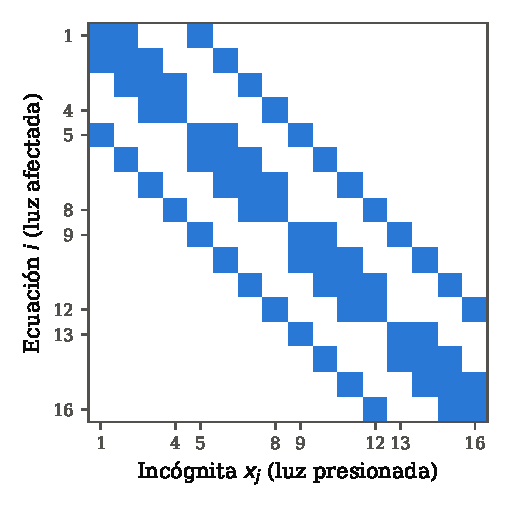
\includegraphics[width=0.48\textwidth]{generado/figura_matriz_4x4.pdf}
  \caption{Matriz $A$ del sistema para un tablero de $4\times 4$. Cada casilla azul es un 1: la fila $i$ es la ecuación de la luz $i$ y la columna $j$ es la incógnita de la luz $j$, con las luces numeradas por filas. La diagonal principal corresponde a la luz presionada, las diagonales vecinas a sus vecinas de la misma fila y las diagonales a distancia 4 a sus vecinas de la fila de arriba y de abajo.}
  \label{fig:matriz}
\end{figure}

Para el tablero $3\times 3$ de la consigna,
\[
T=\begin{pmatrix}0&1&0\\1&1&0\\0&0&1\end{pmatrix},\qquad
\begin{array}{ccc}x_1 & x_2 & x_3\\ x_4 & x_5 & x_6\\ x_7 & x_8 & x_9\end{array}
\]
donde a la derecha se indica la incógnita que corresponde a cada posición. La Tabla~\ref{tab:ecuaciones} detalla la construcción de cada una de las nueve ecuaciones. La luz $a_{11}$ es una esquina, por lo que solo la afectan ella misma y sus dos vecinas $a_{12}$ y $a_{21}$; como está apagada, la ecuación es $x_1+x_2+x_4=0$. Del mismo modo, $a_{12}$ está en el borde superior y la afectan $a_{11}$, $a_{12}$, $a_{13}$ y $a_{22}$; como está prendida, debe recibir una cantidad impar de cambios y la ecuación es $x_1+x_2+x_3+x_5=1$. La luz central $a_{22}$ tiene cuatro vecinas y por eso su ecuación es la única con cinco incógnitas. El resto de las ecuaciones se obtiene con el mismo razonamiento.

\begin{table}[H]
\centering
\caption{Construcción de las ecuaciones del sistema para el tablero $3\times 3$ de la consigna}
\label{tab:ecuaciones}
\small
\begin{tabular}{c c l l c l}
\toprule
Ec. & Luz & Ubicación & Luces que la afectan & Estado & Ecuación \\
\midrule
1 & $a_{11}$ & esquina & $a_{11},a_{12},a_{21}$ & 0 & $x_1+x_2+x_4=0$ \\
2 & $a_{12}$ & borde & $a_{11},a_{12},a_{13},a_{22}$ & 1 & $x_1+x_2+x_3+x_5=1$ \\
3 & $a_{13}$ & esquina & $a_{12},a_{13},a_{23}$ & 0 & $x_2+x_3+x_6=0$ \\
4 & $a_{21}$ & borde & $a_{11},a_{21},a_{22},a_{31}$ & 1 & $x_1+x_4+x_5+x_7=1$ \\
5 & $a_{22}$ & centro & $a_{12},a_{21},a_{22},a_{23},a_{32}$ & 1 & $x_2+x_4+x_5+x_6+x_8=1$ \\
6 & $a_{23}$ & borde & $a_{13},a_{22},a_{23},a_{33}$ & 0 & $x_3+x_5+x_6+x_9=0$ \\
7 & $a_{31}$ & esquina & $a_{21},a_{31},a_{32}$ & 0 & $x_4+x_7+x_8=0$ \\
8 & $a_{32}$ & borde & $a_{22},a_{31},a_{32},a_{33}$ & 0 & $x_5+x_7+x_8+x_9=0$ \\
9 & $a_{33}$ & esquina & $a_{23},a_{32},a_{33}$ & 1 & $x_6+x_8+x_9=1$ \\
\bottomrule
\end{tabular}

\vspace{4pt}
\begin{minipage}{0.95\textwidth}
\footnotesize\textit{Nota.} La columna \textit{Estado} es el valor inicial de la luz en el tablero y es el término independiente de la ecuación. La luz $a_{fc}$ corresponde a la incógnita $x_{3(f-1)+c}$.
\end{minipage}
\end{table}

\subsection{Algoritmo de resolución}\label{sec:algoritmo}

Para resolver el sistema se usa la escalerización de Gauss-Jordan sobre la matriz ampliada $[A\,|\,\mathbf{b}]$ con la suma de $\F$. La consigna indica que no es necesario el pivoteo, es decir, que en cada paso la entrada en la posición de pivote ya vale 1. Al implementar el método se comprobó que esto no ocurre (ver Sección~\ref{sec:res_pivoteo}), por lo que el algoritmo incluye el intercambio de filas. El procedimiento se resume en el Algoritmo~\ref{alg:gauss}.

\begin{algorithm}[H]
\caption{Resolución de \textit{Lights Out} por escalerización con suma binaria}
\label{alg:gauss}
\small
\Entrada{tablero $T$ de $n\times n$ con entradas en $\{0,1\}$}
\Salida{vector $\mathbf{x}\in\F^{n^2}$ con las luces a presionar, o aviso de que no hay solución}
Construir $A$ según la Ecuación~\eqref{eq:matriz} y $\mathbf{b}$ recorriendo $T$ por filas\;
$M\leftarrow[A\,|\,\mathbf{b}]$;\quad $f\leftarrow 1$;\quad $P\leftarrow$ lista vacía de columnas pivote\;
\For{$c\leftarrow 1$ \KwTo $n^2$}{
  \If{ninguna fila $k\geq f$ tiene $M_{kc}=1$}{\textbf{continuar} con la siguiente columna ($x_c$ es libre)\;}
  Tomar la primera fila $k\geq f$ con $M_{kc}=1$ e intercambiar $F_k$ y $F_f$ si $k\neq f$\;
  \For{cada fila $i\neq f$ con $M_{ic}=1$}{$F_i\leftarrow F_i+F_f$ \tcp*{suma binaria}}
  Agregar $c$ a $P$;\quad $f\leftarrow f+1$\;
}
\If{alguna fila $i\geq f$ tiene término independiente 1}{\Return{no hay solución} \tcp*{fila $0=1$}}
$\mathbf{x}\leftarrow\mathbf{0}$\;
\For{cada fila $i$ con pivote en la columna $P_i$}{$x_{P_i}\leftarrow$ término independiente de $F_i$\;}
\Return{$\mathbf{x}$}
\end{algorithm}

Como se eliminan los unos por encima y por debajo de cada pivote, al terminar cada fila no nula tiene un único 1 entre las columnas pivote, y la ecuación de esa fila determina el valor de su incógnita pivote una vez fijadas las libres. El algoritmo asigna 0 a las incógnitas libres, de modo que, cuando hay varias soluciones, devuelve una de ellas. Para analizar la cantidad de pulsaciones se implementó además una opción que recorre las $2^{\dim N(A)}$ soluciones, sumando a la solución anterior todas las combinaciones de una base del núcleo, y devuelve una de las que tienen menos unos. La base del núcleo se obtiene de la forma reducida: cada incógnita libre da un vector que vale 1 en ella, 0 en las demás libres y, en cada incógnita pivote, el valor que anula su ecuación.

\subsection{Implementación}\label{sec:implementacion}

El método se implementó en Python~3 con las bibliotecas NumPy (Harris et al., 2020), para el manejo de matrices, y Matplotlib (Hunter, 2007), para las figuras. Las filas se representan como vectores de enteros sin signo de 8 bits, y la operación $F_i\to F_i+F_f$ se calcula con el operador \textit{o exclusivo} (XOR), que coincide con la suma de $\F$ y opera sobre todas las columnas a la vez. El código fuente, las pruebas y las instrucciones para reproducir todos los resultados de este informe se encuentran en el repositorio \url{\repositorio}. El repositorio contiene tres archivos:
\begin{itemize}[leftmargin=2em,itemsep=0pt]
  \item \codigo{lights\_out.py}: módulo con el modelo y la función pedida, \codigo{resolver\_lights\_out}, que recibe una matriz $n\times n$ de ceros y unos y devuelve el vector solución, o lanza la excepción \codigo{SinSolucionError} si el tablero no tiene solución. Incluye también una simulación del juego (\codigo{presionar}, \codigo{aplicar\_solucion}) que aplica las reglas directamente sobre el tablero, sin usar la matriz $A$.
  \item \codigo{test\_lights\_out.py}: pruebas automáticas que comparan el sistema construido con el de la consigna, verifican la jugada de ejemplo sobre $a_{43}$ y comprueban las soluciones obtenidas.
  \item \codigo{experimentos.py}: genera todas las tablas y figuras de la Sección~\ref{sec:resultados} y un archivo con los resultados numéricos.
\end{itemize}

\subsection{Diseño de las pruebas y criterios de análisis}\label{sec:pruebas}

Se usaron cuatro conjuntos de casos. El primero son los ejemplos de la consigna: el tablero $3\times 3$, cuyo sistema y solución se compararon con los dados, y el tablero $5\times 5$ usado para ilustrar una jugada. El segundo es un tablero $3\times 3$ tomado de una captura del juego en línea Grid Lights (Artbylogic, s.f.), en el que se interpretó una luz verde como prendida y una roja como apagada. El tercero son tableros aleatorios: para cada $n$ entre 1 y 10 se generaron 2000 tableros con entradas independientes que valen 0 o 1 con igual probabilidad. El cuarto son 200 tableros con solución para cada $n\in\{4,5,9\}$, generados como $\mathbf{b}=A\mathbf{z}$ con $\mathbf{z}$ aleatorio, que se usaron para comparar la cantidad de pulsaciones de las soluciones. Todos los tableros aleatorios se obtuvieron de un único generador de números pseudoaleatorios inicializado con la semilla 2026, de modo que los resultados son reproducibles.

Se aplicaron los siguientes criterios. Una solución se consideró correcta si, al aplicarla con la simulación del juego, el tablero queda completamente apagado; como la simulación no usa la matriz $A$, esta comprobación es independiente de la construcción del sistema. Para cada $n$ se registraron el rango de $A$ y la dimensión de su núcleo, y se comparó la fracción observada de tableros con solución con la fracción teórica $2^{r}/2^{n^2}=2^{-\dim N(A)}$, que resulta de que la imagen de $A$ tiene $2^r$ elementos. Por último, para evaluar la indicación de la consigna sobre el pivoteo, se escalerizó la matriz $A$ en el orden natural de las ecuaciones sin intercambiar filas y se registró el primer paso en que el elemento de la diagonal es 0.

% ---------------------------------------------------------------------------
\section{Resultados}\label{sec:resultados}
% ---------------------------------------------------------------------------

\subsection{Ejemplo de la consigna}\label{sec:res_ejemplo}

La matriz $A$ y el vector $\mathbf{b}$ construidos por el programa para el tablero $3\times 3$ coinciden ecuación por ecuación con el sistema de la consigna, y la función devolvió el vector $\mathbf{x}=(0,0,0,0,1,0,0,0,1)$, es decir, $x_5=x_9=1$, que corresponde a presionar las luces $a_{22}$ y $a_{33}$. La Tabla~\ref{tab:verificacion} muestra la sustitución de esta solución en cada ecuación: en todos los casos el lado izquierdo coincide con el término independiente. En las ecuaciones 6 y 8 aparecen a la vez $x_5$ y $x_9$, y la suma $1+1=0$ refleja que las luces $a_{23}$ y $a_{32}$ cambian dos veces de estado.

\begin{table}[H]
\centering
\caption{Verificación de la solución $x_5=x_9=1$, $x_i=0$ en las demás incógnitas, para el tablero $3\times 3$}
\label{tab:verificacion}
\small
\begin{tabular}{c l l c c}
\toprule
Ec. & Ecuación & Sustitución & Resultado & Término independiente \\
\midrule
1 & $x_1+x_2+x_4$ & $0+0+0$ & 0 & 0 \\
2 & $x_1+x_2+x_3+x_5$ & $0+0+0+1$ & 1 & 1 \\
3 & $x_2+x_3+x_6$ & $0+0+0$ & 0 & 0 \\
4 & $x_1+x_4+x_5+x_7$ & $0+0+1+0$ & 1 & 1 \\
5 & $x_2+x_4+x_5+x_6+x_8$ & $0+0+1+0+0$ & 1 & 1 \\
6 & $x_3+x_5+x_6+x_9$ & $0+1+0+1$ & 0 & 0 \\
7 & $x_4+x_7+x_8$ & $0+0+0$ & 0 & 0 \\
8 & $x_5+x_7+x_8+x_9$ & $1+0+0+1$ & 0 & 0 \\
9 & $x_6+x_8+x_9$ & $0+0+1$ & 1 & 1 \\
\bottomrule
\end{tabular}

\vspace{4pt}
\begin{minipage}{0.95\textwidth}
\footnotesize\textit{Nota.} Las sumas se calculan en $\{0,1\}$ con $1+1=0$.
\end{minipage}
\end{table}

Para este tablero la escalerización no dejó incógnitas libres (rango 9), por lo que esta es la única solución del sistema. La primera fila de la Figura~\ref{fig:ejemplos} muestra el tablero inicial, las luces presionadas y el tablero final obtenido con la simulación.

\subsection{Captura del juego en línea y tablero 5\texorpdfstring{$\times$}{x}5 de la consigna}

Para el tablero de la captura de Grid Lights,
\[
T=\begin{pmatrix}0&1&1\\0&0&1\\0&0&0\end{pmatrix},
\]
la función devolvió $\mathbf{x}=(0,0,1,0,0,0,0,0,0)$, es decir, presionar únicamente la luz $a_{13}$. Al ser también un tablero $3\times 3$, la solución es única. La segunda fila de la Figura~\ref{fig:ejemplos} muestra el resultado.

\begin{figure}[H]
  \centering
  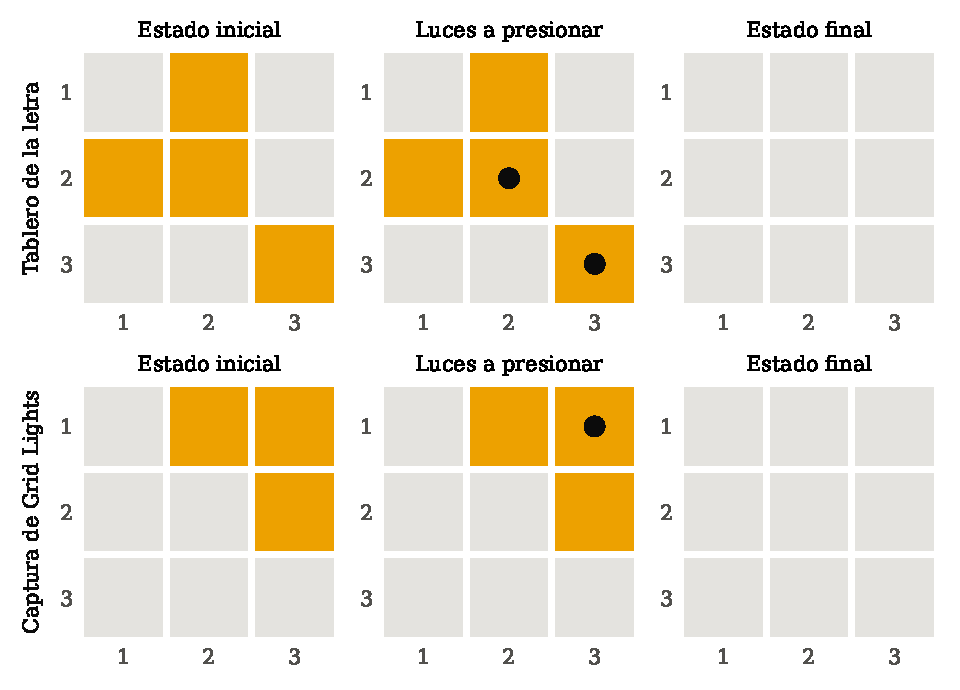
\includegraphics[width=0.85\textwidth]{generado/figura_ejemplos.pdf}
  \caption{Resolución de los dos tableros $3\times 3$: arriba, el ejemplo de la consigna; abajo, la captura del juego Grid Lights. Las casillas amarillas son luces prendidas y las grises, apagadas. La columna central marca con un punto negro las luces que indica presionar la función \codigo{resolver\_lights\_out}, y la columna derecha es el tablero que resulta de presionarlas según las reglas del juego.}
  \label{fig:ejemplos}
\end{figure}

La simulación de la jugada sobre $a_{43}$ en el tablero $5\times 5$ de la consigna reprodujo exactamente el tablero que se muestra allí. Sin embargo, el sistema asociado a ese tablero resultó incompatible: la escalerización produjo una fila de la forma $0=1$, de modo que ese estado no puede apagarse. Para $n=5$ el núcleo de $A$ tiene dimensión 2 y una base es
\[
\mathbf{z}_1=\begin{pmatrix}0&1&1&1&0\\1&0&1&0&1\\1&1&0&1&1\\1&0&1&0&1\\0&1&1&1&0\end{pmatrix},\qquad
\mathbf{z}_2=\begin{pmatrix}1&0&1&0&1\\1&0&1&0&1\\0&0&0&0&0\\1&0&1&0&1\\1&0&1&0&1\end{pmatrix},
\]
escritos como tableros. El producto (con la suma de $\F$) del vector $\mathbf{b}$ de ese tablero con $\mathbf{z}_1$ es 1 y con $\mathbf{z}_2$ es 0.

\subsection{Estructura del sistema según el tamaño del tablero}

La Tabla~\ref{tab:tamanos} resume, para cada $n$ entre 1 y 10, el rango de $A$, la dimensión de su núcleo, la fracción de tableros con solución esperada y la observada en los 2000 tableros aleatorios, y la cantidad de soluciones que apagaron el tablero en la simulación. La matriz tiene rango completo para $n\in\{1,2,3,6,7,8,10\}$, y en esos tamaños todos los tableros generados tuvieron solución. Para $n=4$, $n=5$ y $n=9$ el núcleo tiene dimensión 4, 2 y 8, respectivamente, y la proporción de tableros con solución fue de 0,0615, 0,2475 y 0,0035, frente a los valores teóricos 0,0625, 0,25 y 0,0039. En todos los tamaños, el 100\,\% de las soluciones devueltas por la función apagó el tablero al aplicarse con la simulación. La Figura~\ref{fig:fraccion} representa la comparación entre ambas fracciones.

\begin{table}[H]
\centering
\caption{Rango y núcleo de la matriz del sistema, y fracción de tableros aleatorios con solución, para $n$ entre 1 y 10}
\label{tab:tamanos}
\small
\begin{tabular}{c c c c c c c c}
\toprule
$n$ & Incógnitas & Rango & $\dim N(A)$ & \multicolumn{2}{c}{Fracción con solución} & Soluciones & Paso con \\
\cmidrule(lr){5-6}
 & ($n^2$) & de $A$ & & Teórica & Observada & verificadas & pivote nulo \\
\midrule
\filasdetabla{generado/tabla_tamanos.tex}
\bottomrule
\end{tabular}

\vspace{4pt}
\begin{minipage}{0.95\textwidth}
\footnotesize\textit{Nota.} La fracción teórica es $2^{-\dim N(A)}$. La fracción observada se calculó sobre 2000 tableros aleatorios por tamaño (semilla 2026). \textit{Soluciones verificadas} indica cuántas de las soluciones obtenidas apagaron el tablero en la simulación, sobre el total de tableros con solución. \textit{Paso con pivote nulo} es el primer paso de la escalerización sin intercambio de filas en el que la entrada diagonal es 0; un guion indica que ese caso no se presenta.
\end{minipage}
\end{table}

\begin{figure}[H]
  \centering
  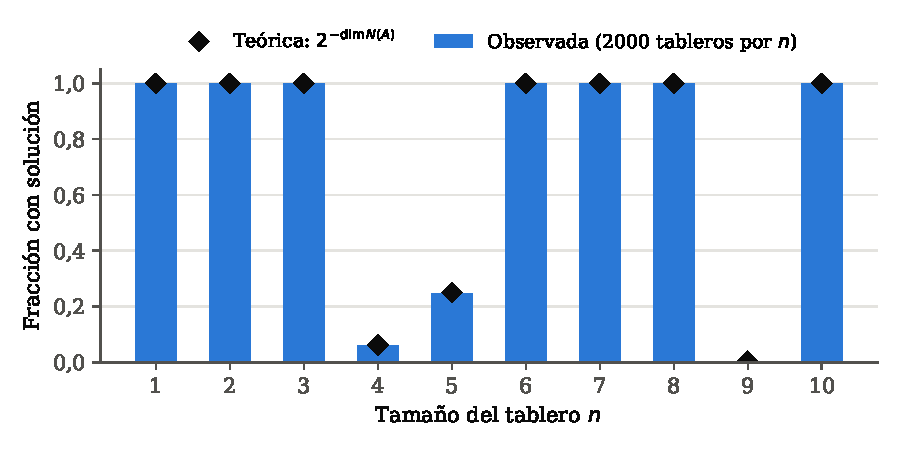
\includegraphics[width=0.85\textwidth]{generado/figura_fraccion.pdf}
  \caption{Fracción de tableros $n\times n$ que tienen solución. Las barras muestran la proporción observada en 2000 tableros aleatorios por tamaño y los rombos, el valor teórico $2^{-\dim N(A)}$. Para $n=9$ la proporción es 0,0035, por lo que la barra no es visible a esta escala.}
  \label{fig:fraccion}
\end{figure}

\subsection{Escalerización sin intercambio de filas}\label{sec:res_pivoteo}

Al escalerizar $A$ en el orden natural de las ecuaciones sin intercambiar filas, la entrada diagonal del segundo paso fue 0 para todos los tamaños entre $n=2$ y $n=10$ (última columna de la Tabla~\ref{tab:tamanos}). Para $n=3$, las dos primeras filas de $A$ son
\[
F_1=(1,1,0,1,0,0,0,0,0),\qquad F_2=(1,1,1,0,1,0,0,0,0),
\]
y la eliminación de la primera columna, $F_2\to F_2+F_1$, da $F_2=(0,0,1,1,1,0,0,0,0)$, cuya segunda entrada es 0. La fila $F_3=(0,1,1,0,0,1,0,0,0)$ sí tiene un 1 en esa columna, por lo que un intercambio de filas permite continuar. En la implementación con intercambio, la escalerización de $A$ requirió entre 1 y 41 intercambios de filas según el tamaño (1 para $n=2$, 3 para $n=3$ y 41 para $n=10$).

\subsection{Cantidad de pulsaciones}

La Tabla~\ref{tab:pulsaciones} compara, para los tamaños con más de una solución por tablero, la cantidad media de luces que presiona la solución con incógnitas libres en 0 y la de la solución con menos pulsaciones. En los tres tamaños la solución mínima requirió en promedio menos pulsaciones: 4,22 frente a 6,20 para $n=4$, 9,91 frente a 11,22 para $n=5$ y 27,79 frente a 36,64 para $n=9$.

\begin{table}[H]
\centering
\caption{Cantidad media de luces presionadas por la solución con incógnitas libres en 0 y por la solución mínima}
\label{tab:pulsaciones}
\small
\begin{tabular}{c c c c c}
\toprule
$n$ & $\dim N(A)$ & Tableros & \multicolumn{2}{c}{Pulsaciones medias} \\
\cmidrule(lr){4-5}
 & & & Libres en 0 & Mínima \\
\midrule
\filasdetabla{generado/tabla_pulsaciones.tex}
\bottomrule
\end{tabular}

\vspace{4pt}
\begin{minipage}{0.95\textwidth}
\footnotesize\textit{Nota.} Tableros con solución generados como $A\mathbf{z}$ para $\mathbf{z}$ aleatorio (semilla 2026). Cada tablero admite $2^{\dim N(A)}$ soluciones.
\end{minipage}
\end{table}

% ---------------------------------------------------------------------------
\section{Discusión}\label{sec:discusion}
% ---------------------------------------------------------------------------

Los resultados confirman que el modelo lineal describe correctamente el juego. El sistema generado por el programa coincide con el de la consigna, la solución $x_5=x_9=1$ satisface las nueve ecuaciones y todas las soluciones obtenidas para tableros aleatorios apagaron el tablero en una simulación que no depende de la matriz $A$. Esto último es relevante porque un error en la construcción de $A$ (por ejemplo, en la numeración de las luces o en el tratamiento de los bordes) produciría soluciones que satisfacen el sistema pero no ganan el juego, y la comparación con la simulación lo habría detectado.

El hallazgo más importante es que la existencia de solución depende del tamaño del tablero. Cuando $A$ es invertible, cada tablero tiene exactamente una solución; cuando no lo es, la imagen de $A$ es un subespacio propio de $\F^{n^2}$ y solo los tableros que pertenecen a ella pueden apagarse. Para $n=5$ el rango es 23, lo que coincide con lo reportado por Anderson y Feil (1998), y solo uno de cada cuatro tableros tiene solución. Las frecuencias observadas en la Tabla~\ref{tab:tamanos} difieren de las teóricas en a lo sumo 0,0025, una diferencia menor que el error estándar de una proporción estimada con 2000 tableros (aproximadamente 0,01 para $n=5$), por lo que el acuerdo entre teoría y experimento es el esperable. El caso $n=9$ muestra que el tamaño del núcleo no crece de forma regular con $n$: allí solo 7 de los 2000 tableros tuvieron solución, mientras que para $n=10$ la tuvieron todos.

El tablero $5\times 5$ de la consigna ilustra este fenómeno. La consigna lo usa solamente para mostrar una jugada, pero ese estado no tiene solución. Como $A$ es simétrica, su imagen coincide con el conjunto de vectores ortogonales (con la suma de $\F$) a todos los vectores de su núcleo (Anderson y Feil, 1998), y por eso basta comprobar dos productos: el producto con $\mathbf{z}_1$ es 1, lo que muestra que el tablero no está en la imagen. Este criterio tiene una interpretación concreta. Presionar las luces marcadas en $\mathbf{z}_1$ no cambia ningún tablero, y el producto $\mathbf{z}_1\cdot\mathbf{b}$ cuenta, módulo 2, las luces prendidas en las posiciones marcadas por $\mathbf{z}_1$. Toda pulsación cambia una cantidad par de esas luces, por lo que la paridad se conserva durante todo el juego; si al comienzo es impar, nunca se llega al tablero apagado, cuya paridad es par. Además, como la jugada sobre $a_{43}$ suma a $\mathbf{b}$ una columna de $A$, que pertenece a la imagen, el tablero resultante tampoco tiene solución.

En cuanto al método, la indicación de la consigna de que nunca es necesario el pivoteo no se verificó en este trabajo. Para todo $n\geq 2$ las luces 1 y 2 son vecinas, por lo que las dos primeras filas de $A$ tienen un 1 en las columnas 1 y 2; al sumar $F_1$ a $F_2$ ambas entradas se anulan, y el segundo pivote resulta 0. Una implementación que asumiera que el pivote siempre es 1 cometería un error a partir del segundo paso. Una interpretación posible es que la consigna se refiere a que, en $\F$, no hay que elegir el pivote de mayor valor absoluto para reducir errores de redondeo, como se hace con números reales, ya que todas las operaciones son exactas; en ese sentido es cierto que no se necesita una estrategia de pivoteo, pero sigue siendo necesario intercambiar filas cuando el elemento en la posición de pivote es 0.

Cuando hay varias soluciones, la elección de las incógnitas libres afecta la cantidad de pulsaciones, como muestra la Tabla~\ref{tab:pulsaciones}. Asignar 0 a las incógnitas libres es una elección cómoda, pero no produce la solución más corta: en $n=4$ la solución mínima requiere en promedio alrededor de un tercio menos de pulsaciones. Obtener la mínima exige recorrer las $2^{\dim N(A)}$ soluciones, lo que es posible para los tamaños estudiados pero crece exponencialmente con la dimensión del núcleo.

El trabajo tiene algunas limitaciones. La escalerización requiere del orden de $n^6$ operaciones elementales, ya que procesa una matriz de $n^2\times n^2$ con hasta $n^2$ eliminaciones por columna; esto es suficiente para los tamaños usados en el juego, pero sería lento para tableros mucho más grandes, en los que convendría aprovechar que $A$ es dispersa. Los resultados empíricos se limitan a $n\leq 10$ y a una única semilla. Por último, para la captura de Grid Lights se supuso que la luz verde está prendida; si se usara la convención opuesta, el tablero inicial sería el complemento y la solución cambiaría, aunque el método sería el mismo.

% ---------------------------------------------------------------------------
\section{Conclusiones}\label{sec:conclusiones}
% ---------------------------------------------------------------------------

Se mostró que el juego \textit{Lights Out} admite un modelo lineal exacto. Como presionar dos veces una luz no tiene efecto y el orden de las pulsaciones no altera el resultado, cada solución se representa con un vector de $\F^{n^2}$, y apagar el tablero equivale a resolver el sistema $A\mathbf{x}=\mathbf{b}$, donde $A$ codifica los vecindarios de las luces y $\mathbf{b}$ el estado inicial. Para el ejemplo $3\times 3$ de la consigna se justificaron las nueve ecuaciones y se verificó que presionar $a_{22}$ y $a_{33}$ es su única solución.

La función implementada en Python resuelve el sistema mediante escalerización de Gauss-Jordan con suma binaria y resolvió correctamente todos los tableros con solución que se le presentaron. Para que funcione en todos los casos fue necesario incluir el intercambio de filas, contrariamente a lo indicado en la consigna, y detectar los sistemas incompatibles.

En cuanto al cuarto objetivo, se concluye que todo tablero tiene solución única cuando la matriz del sistema es invertible, lo que ocurre para $n\in\{1,2,3,6,7,8,10\}$ dentro de los tamaños estudiados. Para $n\in\{4,5,9\}$ solo una fracción $2^{-\dim N(A)}$ de los tableros tiene solución, y cada uno de ellos admite $2^{\dim N(A)}$ soluciones distintas. El mismo análisis permite decidir antes de jugar si un tablero tiene solución, comprobando su paridad respecto de los vectores del núcleo, como se mostró con el tablero $5\times 5$ de la consigna.

Como líneas de trabajo futuro, se propone aprovechar la estructura dispersa de $A$ para resolver tableros de mayor tamaño, estudiar con mayor generalidad para qué valores de $n$ la matriz es invertible y extender el modelo a variantes del juego, como tableros rectangulares o luces con más de dos estados, en las que la suma se calcula módulo un número mayor.

% ---------------------------------------------------------------------------
\section*{Referencias}
% ---------------------------------------------------------------------------
\addcontentsline{toc}{section}{Referencias}

\begingroup
\setlength{\parindent}{-1.27cm}
\setlength{\leftskip}{1.27cm}
\setlength{\parskip}{0.5em}

Anderson, M., y Feil, T. (1998). Turning lights out with linear algebra. \textit{Mathematics Magazine, 71}(4), 300--303. \url{https://doi.org/10.1080/0025570X.1998.11996658}

Artbylogic. (s.f.). \textit{Grid Lights} [Juego en línea]. \url{https://artbylogic.com}

Harris, C. R., Millman, K. J., van der Walt, S. J., Gommers, R., Virtanen, P., Cournapeau, D., Wieser, E., Taylor, J., Berg, S., Smith, N. J., Kern, R., Picus, M., Hoyer, S., van Kerkwijk, M. H., Brett, M., Haldane, A., Fernández del Río, J., Wiebe, M., Peterson, P., \ldots{} Oliphant, T. E. (2020). Array programming with NumPy. \textit{Nature, 585}(7825), 357--362. \url{https://doi.org/10.1038/s41586-020-2649-2}

Hunter, J. D. (2007). Matplotlib: A 2D graphics environment. \textit{Computing in Science \& Engineering, 9}(3), 90--95. \url{https://doi.org/10.1109/MCSE.2007.55}

Lay, D. C., Lay, S. R., y McDonald, J. J. (2016). \textit{Linear algebra and its applications} (5.ª ed.). Pearson.

Lidl, R., y Niederreiter, H. (1997). \textit{Finite fields} (2.ª ed.). Cambridge University Press.

Universidad Católica del Uruguay. (s.f.). \textit{Proyecto Lights Out!} [Consigna del curso Álgebra Aplicada]. Facultad de Ingeniería y Tecnologías.

\endgroup

\end{document}
